\section{Background}
\label{section:background}

\subsection{Hardware}

An exoskeleton is a wearable mechanical device that augments the user's performance, often to aid the user in certain positions or activities \cite{exodefinition}. This type of device can be divided into two
categories, active and passive. While passive exoskeletons do not make use of external power sources and use materials
such as springs or dampers, active ones employ one or more actuators (e.g., motors) to assist the user \cite{passiveactiveexo}.


\subsection{Electromyography}

\subsubsection{Electromyography}

The movement of the human body involves numerous electric signals. These electric currents are generated by the brain and sent through the body through the neural network
to contract the muscles and travel through motor neurons until they reach the motor unit, which is composed of the muscle fibers
activated by a single motor neuron \cite{emggen}. To measure these signals, a procedure called \acrfull{emg} is carried out which can use two types of electrodes. \acrfull{semg} 
electrodes that should be placed on the skin above the muscle of interest, or needle electrodes that are placed within the muscle. 

\subsubsection{Surface Electromyography}

Surface electrodes are frequently made out of silver chloride (AgCl), silver (Ag), a silver/silver chloride (Ag/AgCl) mix or gold (Au) \cite{sEMG}.
Silver/Silver chloride electrodes are preferable due to the fact they are almost non-polarizable, meaning that instead of capacitive
they are resistive in regards to the impedance between the skin and the electrode. This provides a highly stable interface with the skin when 
an electrolyte solution is used. Such stability is crucial for the quality of the signal as it lowers the noise and reduces the body-movent generated
artifacts.

\subsubsection{\acrshort{emg} feature extraction}

\acrshort{emg} control systems perform signal analysis on time segments from which usually three types of features are considered \cite{EMGprediction}:
\begin{itemize}
    \item \textbf{Time-domain features:} These are computed from the raw \acrshort{emg} and involve a lower computation cost than the other types of features,
    which is the reason why they are widely used in classification and regression models. These features include \acrfull{mav}, \acrfull{rms}, \acrfull{zc}, \acrfull{ssc} and \acrfull{wl}
    among others.
    \item \textbf{Frequency-domain features:} some of the most common features extracted from the frequency domain are the \acrfull{ps}, \acrfull{mnf} and \acrfull{fr}.
    These, however, involve a higher computational cost than the time-domain features.
    \item \textbf{Time-frequency domain features:} these features can localize the energy of the signal both in time and frequency, but they usually
    require a transformation that increases the computational cost, as it happens with the \acrfull{stft} or the \acrfull{wt}.
\end{itemize}


\subsection{Sequence models}

\subsubsection{Recurrent Neural Networks}
\acp{rnn} are a type of neural network designed for processing sequences since by using cycles within the network, a \acrshort{rnn} can maintain a state that
represents information about the sequence it has seen so far \cite{RNNdef}. This makes them ideal for tasks such as continuous motion prediction from \acrshort{emg} signals
as the network can learn patterns from the raw data without the need for previous feature extraction as it is done within the model.
In figure \ref{fig:rnn_basic} the basic structure of a \acrshort{rnn} can be seen, where an input is processed and the output is fed again as an input.
Research such as \cite{RNNEMG} has shown that \acp{rnn} can be used to predict continuous motion from \acrshort{emg} signals with a degree of 
accuracy as high as 98.46\%.

\begin{figure}[h]
    \centering
    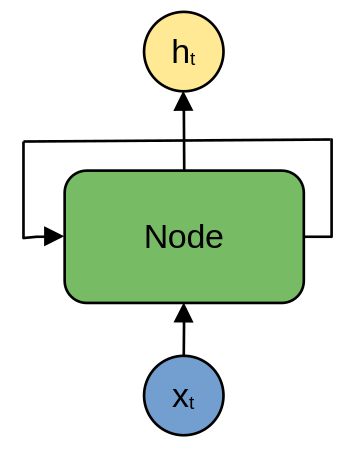
\includegraphics[scale=0.20]{images/rnn_basic.png}
    \caption{Basic structure of a \acrshort{rnn}}
    \label{fig:rnn_basic}
\end{figure}

\subsubsection{Long Short-Term Memory}
\acrfull{lstm} networks were invented to solve the vanishing gradient problem that \acrshort{rnn} networks have by incorporating non-linear data-dependent controls 
into a \acrshort{rnn} cell. In order to achieve this, multiplicative input and output gates were added to protect the memory contents from perturbation of irrelevent inputs
and to protect other units from irrelevant memory contents respectively \cite{LSTMoriginal}.
These \acrshort{lstm} cells present a key weakness, the cell states tend to grow linearly when processing a time series, which can lead to a loss of information as the cell
would stop working as a memory. To solve this issue, forget gates were introduced by Gers et al. \cite{LSTMforget}. These gates are designed to learn to reset memory blocks
when the information they store is no longer relevant. These resets are a gradual reset that corresponds to slowly fading cell states.
In figure \ref{fig:lstm_cell} the structure of a \acrshort{lstm} cell can be seen with its different gates and the activation functions they use and how they cell and hidden states
are calculated.

\begin{figure}[h]
    \centering
    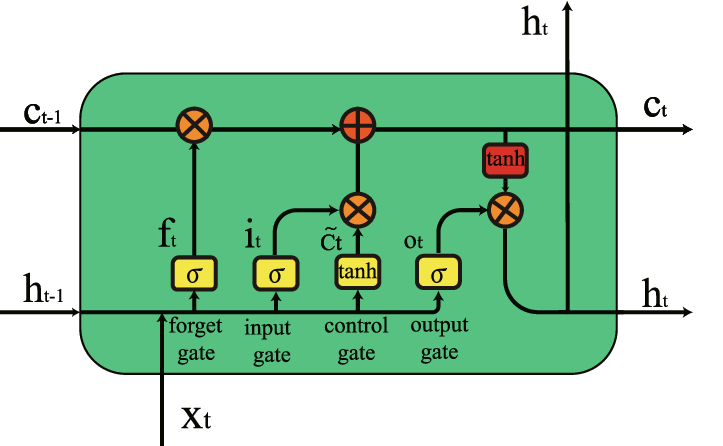
\includegraphics[scale=0.20]{images/lstm_cell.png}
    \caption{Structure of a \acrshort{lstm} cell}
    \label{fig:lstm_cell}
\end{figure}

\subsection{Related Works}
\acrshort{afes} \cite{AFES} achieved a working exoskeleton that could be driven by the bicep. However, the resulting 
exoskeleton presented some limitations. The exoskeleton was mounted on a stand, rendering it therefore unwearable. Another significant limitation 
that the exoskeleton exhibits lies in the fact that it can only be driven by the bicep. As such, the exoskeleton can only show three different states, 
with them being fully extended, fully contracted, and at rest. One key issue that made the exoskeleton a valuable proof of concept, but not a viable 
product consists of the limitations of the hardware and software used. The \acrshort{emg} sensor used employed an outdated Bluetooth module and the software was 
written in Python, which due to its performance is not suitable for real-time applications in such limited hardware. 
\\
One study by Zhou et al. \cite{shoulderexo}, worked on a 12-channel shoulder sEMG system with the use of machine learning techniques. Through the testing, they used Delsys EMG sensors, LABVIEW with ML toolbox and an 
upper limb exoskeleton with more than four \acp{dof} where DAQ and Arduino boards were used for motion control. For the recognition of the shoulder motion and the different patterns ANN was used as an 
ML technique. During testing the accuracy of the movement sensors were controlled with the use of eighteen test subjects. The subjects performed several regular daily activities
such as drinking, muscle abduction, resting, forward and backward motions. The results of the project showed that the motion pattern recognition yielded an average accuracy of 87.98\%-99.34\% 
during offline validation and 74\%-98\% during the real-time online testing. In conclusion, the study showed that the ML ANN technique could be used for processing multiple \acrshort{semg} channels
into an Exoskeleton. Different methods of ML techniques could be used for future research  where further testing to check the effectiveness of algorithms including \acrfull{svm},
\acrfull{cnn}, \acrfull{lr}, and more when implemented with real-time limb motion pattern motion recognition.
\\
Another study that is focused more on continuous motion estimation from EMG signals is named "A review on EMG-based motor intention prediction of continuous human upper limb motion for human-robot collaboration"\cite{continuousemg}.
The study reviewed the EMG-based human-robot collaboration system from multiple perspectives they controlled both healthy and disabled users where an offline test was conducted until a desired performance was reached before conducting
real-time tests. The tests that were conducted had many different parameters such as joint angle estimation, velocity, elbow angle, and many more for the different parameters different models were used. 
For velocity, they used a state-space model while they used a back-propagation neural network for the elbow angle. The study showed that while testing multiple challenges came up such as signal acquisition where sEMG
is to be placed on a clean and shaven area for a good connection between muscle and electrode to yield a signal of higher quality. Another challenge that was faced in the study showed that the electrodes could shift or lose contact 
with the targeted muscle which resulted in inaccurate EMG signals these shifts could also cause crosstalk. Signals also differ from user to user. The same user could be different EMG signals during separate recordings which also made it 
harder for the motion intention prediction.